
\documentclass[compress, 10pt]{beamer}
\usepackage[utf8]{inputenc}
\usepackage{multirow}
\usepackage{hyperref}

% ou bien Boadilla avec miniframes
\usetheme{Boadilla}
\useoutertheme{miniframes}
\useinnertheme{circles}

\usepackage{tikz} % to draw circuit of RC model
\usetikzlibrary{babel}
\usetikzlibrary{positioning,backgrounds,fadings,shadows.blur,shadows} % to draw circuit of RC model
\usetikzlibrary{fit,shapes,arrows} % to draw circuit of RC model
\usepackage{circuitikz} % to draw circuit of RC model
\usepackage{graphicx}
%\usepackage[dvipsnames]{xcolor}

\usepackage{tikz}
\tikzstyle{arrow} = [thick,->,>=stealth]
\tikzstyle{startstop} = [circle, minimum width=3cm, minimum height=1cm,text centered, draw=black, fill=red!30]

%\usepackage{animate}

\definecolor{vertLOCIE}{rgb}{0.51372549, 0.6980, 0.015} % vert du LOCIE
\definecolor{alertLOCIE}{rgb}{0.78823529, 0.30980392, 0.65882353}
\definecolor{fontalertLOCIE}{rgb}{0.15686275, 0.05882353, 0.12941176}
\definecolor{alertedtext}{rgb}{0.69803922, 0.54117647, 0.01568627}

\usecolortheme[named=vertLOCIE]{structure}
\setbeamercolor{block title alerted}{bg=alertedtext, fg=fontalertLOCIE}
\setbeamercolor{alerted text}{fg=alertedtext}

%\usecolortheme{seahorse}


%Information to be included in the title page:
\title{Introduction to probabilistic modelling}

\author[S. Rouchier]
{Simon Rouchier\inst{}}

\institute[LOCIE, USMB] % (optional)
{
	\inst{}%
	LOCIE UMR CNRS 5271\\
	Université Savoie Mont-Blanc \\
 simon.rouchier@univ-smb.fr

}

\date{16 mai 2024}

\titlegraphic{\includegraphics[height=0.8cm]{./figures/logoLOCIE.png}\hspace*{1cm}~%
		\includegraphics[height=0.8cm]{./figures/logoUSMB.png}\hspace*{1cm}~%
		\includegraphics[height=0.8cm]{./figures/logoCNRS.png}%
}

% produit un logo sur tous les frames !
%\logo{\includegraphics[height=1cm]{./figures/locie-logo-horiz.png}}

%%%%%%%%%%%%%%%%%%%%%%%%%%%%%%%%%%%%%%%%%%%%%%%%%%%%%%%%%%%%%%%%%%%%%%%%%%%%%%%%%%%%%%%%%%%%%%%%%%%%%%%%%

\begin{document}

\frame{\titlepage}

\section[Background]{Background on probabilistic modelling}

\begin{frame}{Contents}
	\tableofcontents[
  currentsection,
  sectionstyle=show/show,
  %subsectionstyle=show/show/hide
]
\end{frame}

%%%%%%%%%%%%%%%%%%%%%%%%%%%%%%%%%%%%%%%%%%%%%%%%%%%%%%%%%%%%%%%%%%%%%%%%%%%%%%%%%%%%%%%%%%%%%%%%%%%%%%%%%

\begin{frame}{Glossary}

\centering
\includegraphics[width=3cm]{figures/definitions.png}

\raggedright
\textbf{Data analysis}: the process of inspecting, cleansing, transforming, and modeling data to extract useful information and support decision-making.

\vspace{0.5cm}

\textbf{Statistical learning} (machine learning): a set of tools for \textit{understanding data}.

\vspace{0.5cm}

\textbf{Probabilistic modelling} (Bayesian modelling, Bayesian data analysis, Bayesian inference): explicit use of probability for quantifying uncertainty in inferences.

\end{frame}



\begin{frame}{Deterministic vs probabilistic modelling}
Deterministic models: the output is entirely determined by the inputs.

\centering
\includegraphics[height=2.4cm]{./figures/modelling_determinist.png}

\raggedright
Probabilistic models:
\begin{itemize}
    \item Unobserved variables $\theta$ are stochastic.
    \item Interdependence between variables is recorded in a probability distribution.
\end{itemize}

\centering
\includegraphics[height=2.4cm]{./figures/modelling_probabilist.png}

\end{frame}

%%%%%%%%%%%%%%%%%%%%%%%%%%%%%%%%%%%%%%%%%%%%%%%%%%%%%%%%%%%%%%%%%%%%%%%%%%%%%%%%%

\begin{frame}{Deterministic vs probabilistic learning}
\centering
\includegraphics[height=6cm]{./figures/learning_determinist.png}
\end{frame}

%%%%%%%%%%%%%%%%%%%%%%%%%%%%%%%%%%%%%%%%%%%%%%%%%%%%%%%%%%%%%%%%%%%%%%%%%%%%%%%%%

\begin{frame}{Deterministic vs probabilistic learning}
\centering
\includegraphics[height=6cm]{./figures/learning_probabilist.png}
\end{frame}

%%%%%%%%%%%%%%%%%%%%%%%%%%%%%%%%%%%%%%%%%%%%%%%%%%%%%%%%%%%%%%%%%%%%%%%%%%%%%%%%%

\begin{frame}{Bayesian data analysis}

The \textbf{model} is a joint probability distribution for $\theta$ and $y$, written as a product of two densities:

\begin{itemize}
    \item A prior distribution $p(\theta)$ which encodes eventual assumptions regarding model parameters, independently of the observed data.
    \item An observational model $p(y|\theta)$, or data distribution, which describes the relationship between the data $y$ and the model parameters $\theta$;
\end{itemize}

\begin{equation*}
    p(\theta,y) = p(\theta) p(y|\theta)
\end{equation*}

\textbf{Prior predictive distribution}: distribution of the observable $y$ before the data are considered.

\begin{equation*}
    p(y) = \int p(y,\theta)\mathrm{d}\theta = \int p(\theta) p(y|\theta) \mathrm{d}\theta
\end{equation*}

\end{frame}

%%%%%%%%%%%%%%%%%%%%%%%%%%%%%%%%%%%%%%%%%%%%%%%%%%%%%%%%%%%%%%%%%%%%%%%%%%%%%%%%%

\begin{frame}{Bayesian data analysis}

Bayesian statistical conclusions about a parameter $\theta$, or unobserved data $\tilde{y}$, are made in terms of probability statements conditional on the observed value of $y$.

\hspace{0.5cm}

\textbf{Bayesian inference}: conditioning on the known value of the data $y$ using Bayes' rule yields the \textbf{posterior} density.

\begin{equation*}
    p(\theta | y) \propto p(\theta) p(y|\theta) 
\end{equation*}

\textbf{Posterior predictive distribution}: prediction of an unknown observable $\tilde{y}$ conditional on the observed $y$.

\begin{equation*}
    p(\tilde{y}|y) = \int p(\tilde{y},\theta|y) \mathrm{d} \theta = \int p(\tilde{y} |\theta)p(\theta|y) \mathrm{d}\theta
\end{equation*}

\end{frame}

%%%%%%%%%%%%%%%%%%%%%%%%%%%%%%%%%%%%%%%%%%%%%%%%%%%%%%%%%%%%%%%%%%%%%%%%%%%%%%%%%

\section{The three steps of Bayesian data analysis}

\begin{frame}{The three steps of Bayesian data analysis}

Gelman et al. Bayesian Data Analysis

\hspace{0.5cm}

\begin{enumerate}
    \item Setting up a full probability model - a joint probability distribution for all observable and unobservable quantities in a problem.
    \item Conditioning on observed data: calculating and interpreting the appropriate posterior distribution.
    \item Evaluating the fit of the model and the implications of the resulting posterior distribution.
\end{enumerate}

\end{frame}

%%%%%%%%%%%%%%%%%%%%%%%%%%%%%%%%%%%%%%%%%%%%%%%%%%%%%%%%%%%%%%%%%%%%%%%%%%%%%%%%%

\subsection{Setting up a model}

\begin{frame}{Setting up a model}
Setting up a full probability model - a joint probability distribution for all observable and unobservable quantities in a problem. The model should be consistent with knowledge about the underlying scientific problem and the data collection process.
\end{frame}

%%%%%%%%%%%%%%%%%%%%%%%%%%%%%%%%%%%%%%%%%%%%%%%%%%%%%%%%%%%%%%%%%%%%%%%%%%%%%%%%%

\begin{frame}{Setting up a model}

    \begin{columns}
    \column{0.6\textwidth}
        \centering
        \includegraphics[height=5cm]{./figures/olr01.png}
    \column{0.4\textwidth}
    \begin{itemize}
        \item Energy consumption $e$
        \item heating degree days $\mathrm{hdd}$
    \end{itemize}
         
\begin{equation*}
    e_i=a+b \cdot \mathrm{hdd}_i
\end{equation*}
    \end{columns}

\end{frame}

%%%%%%%%%%%%%%%%%%%%%%%%%%%%%%%%%%%%%%%%%%%%%%%%%%%%%%%%%%%%%%%%%%%%%%%%%%%%%%%%%

\begin{frame}{Setting up a model}

    \begin{columns}
    \column{0.6\textwidth}
        \centering
        \includegraphics[height=5cm]{./figures/olr02.png}
    \column{0.4\textwidth}
\begin{align*}
    e_i & =a+b \cdot \mathrm{hdd}_i \\
    a & \sim \mathrm{N}(3000, 100)  \\
    b & \sim \mathrm{N}(1, 0.2) 
\end{align*}
\end{columns}

\end{frame}

%%%%%%%%%%%%%%%%%%%%%%%%%%%%%%%%%%%%%%%%%%%%%%%%%%%%%%%%%%%%%%%%%%%%%%%%%%%%%%%%%

\begin{frame}{Setting up a model}

    \begin{columns}
    \column{0.6\textwidth}
        \centering
        \includegraphics[height=5cm]{./figures/olr03.png}
    \column{0.4\textwidth}
\begin{align*}
    e_i & =a+b \cdot \mathrm{hdd}_i \\
    p(y_i|a,b,\sigma) & = \mathrm{N}(e_i,\sigma) \\ 
    p(a) & = \mathrm{N}(3000, 100) \\
    p(b) & = \mathrm{N}(1, 0.2) \\
    p(\sigma) & = \mathrm{HalfN}(100)
\end{align*}
    \end{columns}

\color{orange}
Prior predictive distribution: $p(y) = \int p(y,\theta)\mathrm{d}\theta = \int p(\theta) p(y|\theta) \mathrm{d}\theta $

\end{frame}

%%%%%%%%%%%%%%%%%%%%%%%%%%%%%%%%%%%%%%%%%%%%%%%%%%%%%%%%%%%%%%%%%%%%%%%%%%%%%%%%%

\subsection{Conditioning on observed data}

\begin{frame}{Conditioning on observed data}
Conditioning on observed data: calculating and interpreting the appropriate posterior distribution - the conditional probability distribution of the unobserved quantities of ultimate interest, given the observed data.

\begin{equation*}
    p(\theta | y) \propto p(\theta) p(y|\theta) 
\end{equation*}
\end{frame}

%%%%%%%%%%%%%%%%%%%%%%%%%%%%%%%%%%%%%%%%%%%%%%%%%%%%%%%%%%%%%%%%%%%%%%%%%%%%%%%%%

\begin{frame}{Conditioning on observed data}
\textbf{Markov Chain Monte Carlo} algorithms:
    \begin{itemize}
        \item Metropolis-Hastings,
        \item Gibbs,
        \item Hamiltonian Monte-Carlo (HMC),
        \item No U-Turn Sampling (NUTS)...
    \end{itemize}

generate a sequence $\left\{\theta^{(1)},...,\theta^{(S)}\right\}$ which approximates the posterior distribution $p(\theta | y)$.

\textbf{Variational Bayesian} methods provide a locally-optimal, exact analytical solution to an approximation of the posterior.
\end{frame}

%%%%%%%%%%%%%%%%%%%%%%%%%%%%%%%%%%%%%%%%%%%%%%%%%%%%%%%%%%%%%%%%%%%%%%%%%%%%%%%%%

\begin{frame}{Conditioning on observed data}
    \begin{columns}
    \column{0.7\textwidth}
        \centering
    \includegraphics[height=5cm]{./figures/olr04.png}
    \column{0.3\textwidth}
\begin{align*}
    p(a) & \rightarrow p(a|y) \\
    p(b) & \rightarrow p(b|y) \\
    p(\sigma) & \rightarrow p(\sigma|y)
\end{align*}
    \end{columns}
    
\centering
\includegraphics[height=1.5cm]{./figures/olr05.png}

\end{frame}

%%%%%%%%%%%%%%%%%%%%%%%%%%%%%%%%%%%%%%%%%%%%%%%%%%%%%%%%%%%%%%%%%%%%%%%%%%%%%%%%%

\begin{frame}{Conditioning on observed data}
$\left\{\theta^{(1)},...,\theta^{(S)}\right\}$ approximates a \textit{joint} distribution of all parameters $p(a,b,\sigma|y)$

\begin{equation*}
    \theta^{(s)} = \left(a,b,\sigma\right)^{(s)}
\end{equation*}

\centering
    \includegraphics[height=5cm]{./figures/olr06.png}
\end{frame}

%%%%%%%%%%%%%%%%%%%%%%%%%%%%%%%%%%%%%%%%%%%%%%%%%%%%%%%%%%%%%%%%%%%%%%%%%%%%%%%%%

\subsection{Evaluating the fit of the model}

\begin{frame}{Evaluating the fit of the model}
Evaluating the fit of the model and the implications of the resulting posterior distribution: how well does the model fit the data, are the substantive conclusions reasonable, and how sensitive are the results to the modeling assumptions in step 1? In response, one can alter or expand the model and repeat the three steps.
\end{frame}

%%%%%%%%%%%%%%%%%%%%%%%%%%%%%%%%%%%%%%%%%%%%%%%%%%%%%%%%%%%%%%%%%%%%%%%%%%%%%%%%%

\begin{frame}{Evaluating the fit of the model}
% https://mc-stan.org/docs/stan-users-guide/posterior-prediction.html
\begin{columns}
    \column{0.5\textwidth}
The posterior predictive density for new data $\tilde{y}$ given observed data $y$ is
\begin{equation*}
    p(\tilde{y}|y) = \int p(\tilde{y},\theta|y) \mathrm{d} \theta = \int p(\tilde{y} |\theta)p(\theta|y) \mathrm{d}\theta
\end{equation*}
    \column{0.5\textwidth}
        \centering
        \includegraphics[height=3cm]{./figures/forecast_probabilist.png}
\end{columns}
Given draws from the posterior $\theta^{(m)} \sim p(\theta|y)$, draws from the posterior predictive $\tilde{y}^{(m)} \sim p(\tilde{y}|y)$ can be generated by randomly generating from the sampling distribution with the parameter draw plugged in,
\begin{equation*}
    \tilde{y}^{(m)} \sim p(y|\theta^{(m)})
\end{equation*}

The posterior distribution or mean of any function $f$ can be approximated as well:

\begin{equation*}
\mathrm{E}\left[f(\tilde{y},\theta)|y\right] \approx \frac{1}{M} \sum_{m=1}^M f(\tilde{y}^{(m)},\theta^{(m)})
\end{equation*}
\end{frame}

%%%%%%%%%%%%%%%%%%%%%%%%%%%%%%%%%%%%%%%%%%%%%%%%%%%%%%%%%%%%%%%%%%%%%%%%%%%%%%%%%


\begin{frame}{Evaluating the fit of the model}
\begin{equation*}
    p(\tilde{y}|y) = \int \underbrace{p(\tilde{y} |\theta)}_{\substack{\textrm{sampling} \\ \textrm{uncertainty}}} \underbrace{p(\theta|y)}_{\substack{\textrm{estimation} \\ \textrm{uncertainty}}} \mathrm{d}\theta
\end{equation*}

\begin{columns}
    \column{0.6\textwidth}
        \centering
        \includegraphics[height=5cm]{./figures/olr07.png}
    \column{0.4\textwidth}
    Estimation uncertainty:
\begin{align*}
    e & = a+b \cdot \mathrm{hdd} \\
    a & \sim p(a|y) \\
    b & \sim p(b|y)
\end{align*}

\color{orange}
Sampling uncertainty:
\begin{align*}
    p(\tilde{y}|a,b,\sigma) & = \mathrm{N}(a+b \cdot \tilde{\mathrm{hdd}},\sigma) \\ 
    \sigma & \sim p(\sigma|y)
\end{align*}
    \end{columns}
    
\end{frame}

%%%%%%%%%%%%%%%%%%%%%%%%%%%%%%%%%%%%%%%%%%%%%%%%%%%%%%%%%%%%%%%%%%%%%%%%%%%%%%%%%

\begin{frame}{Bayesian model comparison and selection}

Given training data $(x,y)$ and test data $(\tilde{x},\tilde{y})$

\centering
\includegraphics[height=3cm]{./figures/forecast_probabilist2.png}

\raggedright
The log pointwise predictive density is a model comparison and selection metric.
    
\begin{equation*}
    \mathrm{log} \, p(\tilde{y}|\tilde{x},x,y) = - \mathrm{log}\, M + \mathrm{logsum exp}_{m=1}^M \mathrm{log}\, p(\tilde{y}|\tilde{x},\theta^{(m)}) 
\end{equation*}

Built-in methods to estimate the expected log pointwise predictive density (elpd) for a new dataset:
\begin{itemize}
    \item Leave-One-Out Cross Validation (LOO-CV)
    \item Widely-applicable Information Criterion (WAIC)
\end{itemize}

% https://www.pymc.io/projects/examples/en/latest/diagnostics_and_criticism/Bayes_factor.html
% https://www.pymc.io/projects/docs/en/stable/learn/core_notebooks/model_comparison.html#model-comparison
% https://mc-stan.org/docs/stan-users-guide/cross-validation.html
% https://mc-stan.org/loo/index.html
\end{frame}


%%%%%%%%%%%%%%%%%%%%%%%%%%%%%%%%%%%%%%%%%%%%%%%%%%%%%%%%%%%%%%%%%%%%%%%%%%%%%%%%%

\section{Increasing model complexity}

\begin{frame}{Contents}
	\tableofcontents[
  currentsection,
  sectionstyle=show/show,
  %subsectionstyle=show/show/hide
]
\end{frame}

\begin{frame}{Measurement and verification}
    \centering
    \includegraphics[width=0.8\textwidth]{figures/mv.png}
\end{frame}


\begin{frame}{M\&V with a change-point model}
    Energy use $y$ as function of ambient temperature $T_a$
    \begin{equation*}
        p(y|\theta,T_a)=\mathrm{Normal}\left[E_0+H_1(T_1-T_a)^++H_2(T_a-T_2)^+,\sigma\right]
    \end{equation*}
    
    \centering
    \includegraphics[width=0.8\textwidth]{figures/changepoint.png}
\end{frame}


\begin{frame}{M\&V with a change-point model}
\centering
\includegraphics[width=0.9\textwidth]{figures/ipmvp_workflow.png}

\end{frame}

\begin{frame}{Autocorrelation}
Problem: correlated prediction residuals denote a biased model.

\centering
    \includegraphics[width=0.45\textwidth]{figures/tuto2corr1-1.png}
    \includegraphics[width=0.45\textwidth]{figures/tuto2corr2-1.png}
\end{frame}

\begin{frame}{Autocorrelation}

Enhancing the original model $f$ with a Moving Average (MA) model
\begin{align*}
    y_n & = f(x_n) + \theta_1 \epsilon_{n-1} + \epsilon_n \\
    \epsilon_n & \sim \mathrm{Normal}(0,\sigma)
\end{align*}

\centering
\includegraphics[width=0.8\textwidth]{figures/movingaverage.PNG}
\end{frame}

\begin{frame}{Autocorrelation}
    \includegraphics[width=0.45\textwidth]{figures/tuto3corr1-1.png}
    \includegraphics[width=0.45\textwidth]{figures/tuto3corr2-1.png}

\begin{itemize}
    \item Decreased model bias
    \item Increased prediction uncertainty and savings uncertainty
\end{itemize}
\end{frame}

\begin{frame}{Time series: ARMAX models}
Autoregressive (AR) model
\begin{equation*}
	y_t \sim N(\alpha + \beta_1 y_{t-1} + \beta_2 y_{t_2} + ... , \sigma^2)
\end{equation*}

\centering
\includegraphics[width=0.4\textwidth]{figures/tikz_ar.png}

\raggedright
AutoRegressive Moving Average with eXogenous inputs
\begin{align*}
	E(y_t|\theta, X) & = \sum_{i=1}^p \beta_i y_{t-i} + \sum_{j=0}^q \gamma_j \varepsilon_{t-j} + \sum_{k=1}^K \left[ \sum_{i=0}^p \theta_{k,i} x_{t-i,k} \right] \\
 \varepsilon_t & \sim N(0,\sigma^2)
\end{align*}
\end{frame}

%%%%%%%%%%%%%%%%%%%%%%%%%%%%%%%%%%%%%%%%%%%%%%%%%%%%%%%%%%%%%%%%%%%%%%

\begin{frame}{Hidden Markov models}

\begin{columns}
    \column{0.5\textwidth}
    \includegraphics[width=\textwidth]{figures/data1.png}
    \column{0.5\textwidth}
    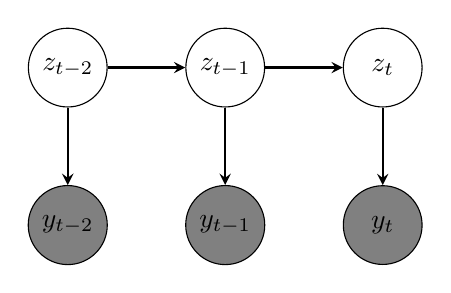
\begin{tikzpicture}[node distance=2cm]
	\node (x1) [circle, minimum size=1cm, fill=white, draw=black, text=black] {$z_{t-2}$};
	\node (x2) [circle, minimum size=1cm, fill=white, draw=black, text=black, right of=x1] {$z_{t-1}$};
	\node (x3) [circle, minimum size=1cm, fill=white, draw=black, text=black, right of=x2] {$z_t$};
\node (y1) [circle, minimum size=1cm, fill=gray, draw=black, text=black, below of=x1] {$y_{t-2}$};
\node (y2) [circle, minimum size=1cm, fill=gray, draw=black, text=black, right of=y1] {$y_{t-1}$};
\node (y3) [circle, minimum size=1cm, fill=gray, draw=black, text=black, right of=y2] {$y_t$};
\draw[arrow] (x1) -- (x2);
\draw[arrow] (x2) -- (x3);
\draw[arrow] (x1) -- (y1);
\draw[arrow] (x2) -- (y2);
\draw[arrow] (x3) -- (y3);
\end{tikzpicture}
\end{columns}

\begin{itemize}
\item The occupancy $z_t$ state at each time $t$ is unknown, and described by a hidden Markov chain with a transition probability matrix:
\begin{equation*}
a_{ij}(h,d)=p\left(z_{h,d}=j |z_{h-1,d}=i\right)
\end{equation*}
\item The energy use $y_t$ follows a different model for each possible occupancy state $z_t$
\begin{equation*}
b_{i}(y_t) = p(y_t|\theta, T_a, z_t=i)
\end{equation*}

\end{itemize}
    
    Rouchier S.  Bayesian Workflow and Hidden Markov Energy-Signature Model for Measurement and Verification. Energies 2022, 15(10), 3534
\end{frame}

%%%%%%%%%%%%%%%%%%%%%%%%%%%%%%%%%%%%%%%%%%%%%%%%%%%%%%%%%%%%%%%%%%%%%%

\begin{frame}{Gaussian Process models}
\begin{columns}
 \column{0.5\textwidth}
Prior distribution over any regression function
\begin{equation*}
    y \sim \mathrm{multivariate}\,\mathrm{normal}\left(m(x),K(x|\theta)\right)
\end{equation*}
    \column{0.5\textwidth}
    \includegraphics[width=\textwidth]{figures/co2.png}
\end{columns}

Gaussian processes are additive and can be used as components in a larger model

\begin{align*}
    y_t(t) & = f_1(t) + f_2(t) + \varepsilon_t \\
    f_1(t) & \sim \mathrm{GP}(0, k_1), \quad k_1(t,t')=\sigma_1^2\mathrm{exp}\left(-\frac{|t-t'|^2}{2 l_1^2}\right) \\
    f_2(t) & \sim \mathrm{GP}(0, k_2), \quad k_2(t,t')=\sigma_2^2\mathrm{exp}\left(-\frac{2\mathrm{sin}^2(\pi(t-t')/7)}{l_2^2}\right) \\
\end{align*}
\end{frame}

%%%%%%%%%%%%%%%%%%%%%%%%%%%%%%%%%%%%%%%%%%%%%%%%%%%%%%%%%%%%%%%%%%%%%%

\begin{frame}{Other models}

\begin{itemize}
    \item Regression models
    \item Time-series models: ARMAX, RC, HMM...
    \item Mixture models
    \item Hierarchical models
    \item Gaussian processes
    \item Missing data, measurement error
\end{itemize}

\end{frame}


%%%%%%%%%%%%%%%%%%%%%%%%%%%%%%%%%%%%%%%%%%%%%%%%%%%%%%%%%%%%%%%%%%%%%%

\section{Material and tools}

\begin{frame}{Material}

Books
\begin{itemize}
    \item Gelman et al. Bayesian Data Analysis
    \item Mc Elreath, Statistical Rethinking
    \item Betancourt, \url{https://betanalpha.github.io/}
\end{itemize}

Probabilistic programming libraries

\begin{tabular}{lll}
  			PyMC & \url{https://www.pymc.io/} & Python \\
		    Stan & \url{https://mc-stan.org/} & Python, R, Julia, Matlab...\\
			Pyro & \url{http://pyro.ai/} & Python \\
\end{tabular}
\end{frame}


\begin{frame}{More content}

\begin{itemize}
    \item This tutorial: \url{https://github.com/srouchier/simurex2024}
    \item \textit{Building energy statistical modelling} book: \url{https://BuildingEnergyGeeks.org/}
    \item Bayesian M\&V: \url{https://srouchier.github.io/bayesmv/}
  
\end{itemize}

\centering
\includegraphics[width=0.6\textwidth]{figures/capture.PNG}

\vspace{.5cm}

\end{frame}

\frame{\titlepage}

\end{document}